\chapter{The LHC and ATLAS Experiment}
\section{The Large Hadron Collider}
The \gls{LHC} \cite{lhc} is a hadron accelerator and collider 27 km in circumference located on the French-Swiss border. It collides beams of protons\footnote{The lhc also collides ions to study lead-lead (PbPb) interactions} at high rate and center-of-mass energy in order to . In ``Run 2,'' the center-of-mass energy was 13 TeV (6.5 TeV per beam), and bunches of about $10^11$ protons collided every 25 ns.

The protons are created by ionizing hydrogen atoms using an electric field, then pass through several accelerators, which take advantage of \gls{RF} cavities to get to their final energy. First, the \gls{Linac} accelerates the bunches to 50 MeV, which then passes bunches to the \gls{PSB}. The remainder of the acceleration chain are all cricular accelerators, starting with the \gls{PSB}, which raises the energy to 1.4 GeV then passes to the \gls{PS}. The \gls{PS}, accelerates bunches to 26 GeV, then the \gls{SPS} accelerates them to 450 GeV before finally delivering to the \gls{LHC}, where they're accelerated to their ultimate energy of 6.5 TeV.


Along the \gls{LHC}, collisions occur at four interaction points, where detectors are situated. LHCb (Large Hadron Collider beauty) is a forward physics experiment studying b physics \cite{lhcb}. ALICE (A Large Ion Collider Experiment) is a heavy-ion detector studying nuclear physics \cite{alice}. The ATLAS \cite{atlas-experiment} and \gls{CMS} \cite{cms} experiments are general-purpose detectors, serving to study a variety of physics. A schematic of the location of these interaction points can be found in figure \ref{fig:lhc}

\begin{figure}
    \centering
    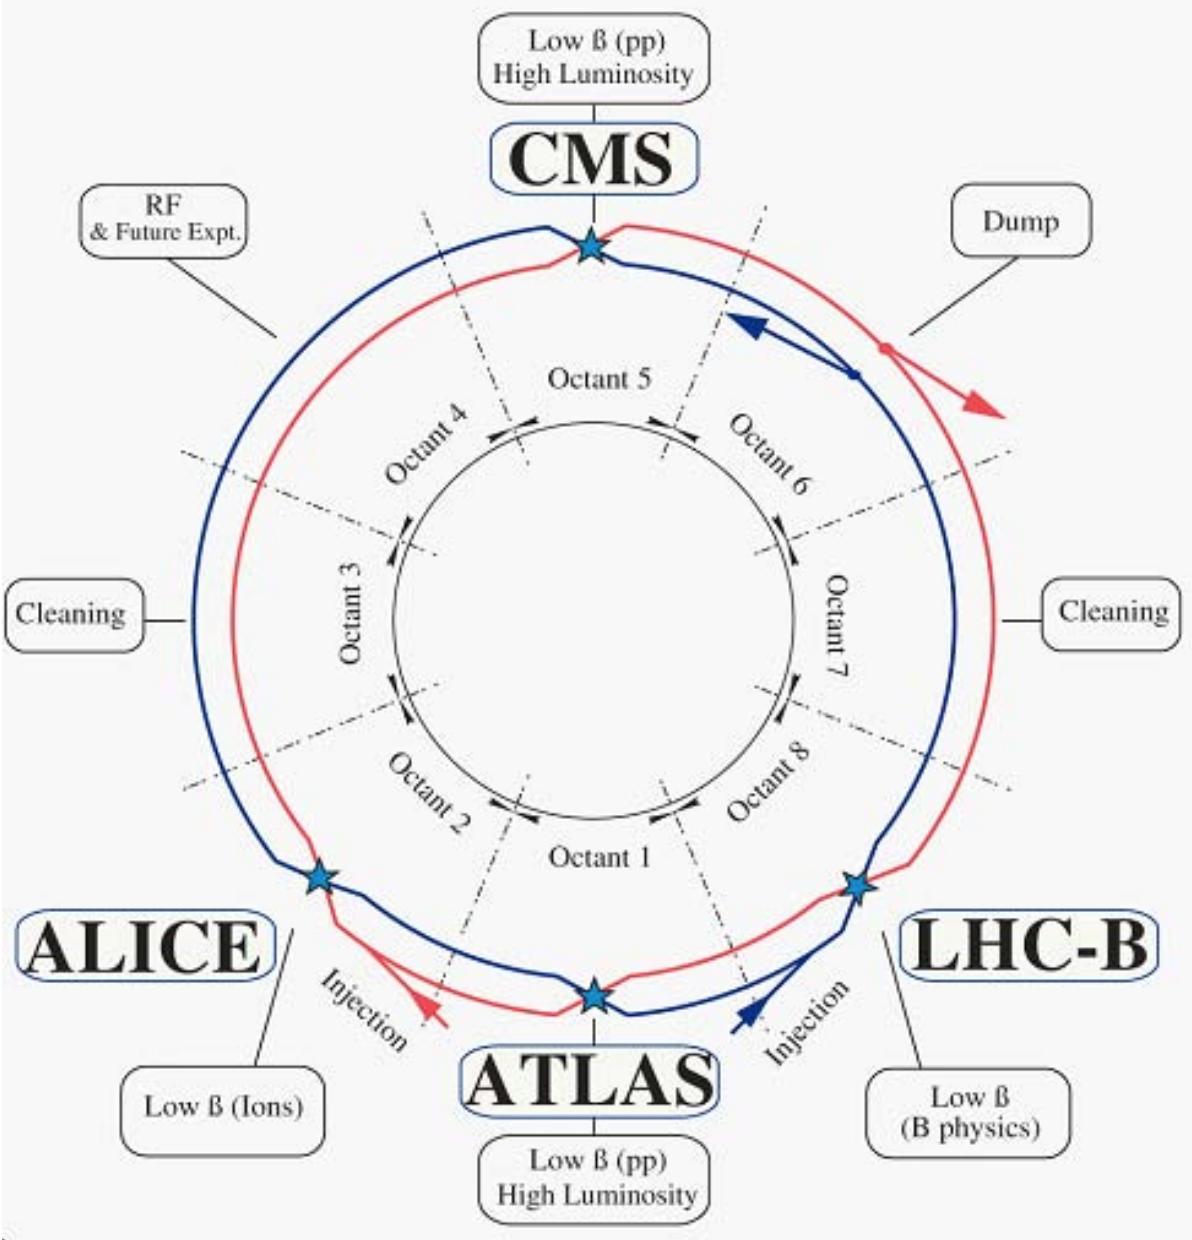
\includegraphics[width=.7\textwidth]{chapters/chapter2_experiment/images/lhc_interaction_points.png}
    \caption{A schematic of the LHC with the various interaction points indicated \cite{lhc}.}
    \label{fig:lhc}
\end{figure}



\section{The ATLAS Detector}
\subsection{Magnet System}
In order to measure the charge and momentum of particles in the detector, a magnetic field is induced. Through the curvature of a charged particle track, the charge to mass ratio can be derived. The sign of the charge is determined from the direction of the track.

The magnet system in ATLAS is a hybrid system comprised of four superconducting magnets: a central solenoid, a barrel toroid, and two end-cap toroids. The barrel toroids define the dimensions of the system, extending 26 m along the beam axis, and has an outer diameter of 22 m
\cite{magnet-system-tdr}. A schematic of the components magnet system is shown in Figure \ref{fig:magnetSystem}.

% Insert picture
\begin{figure}
    \centering
    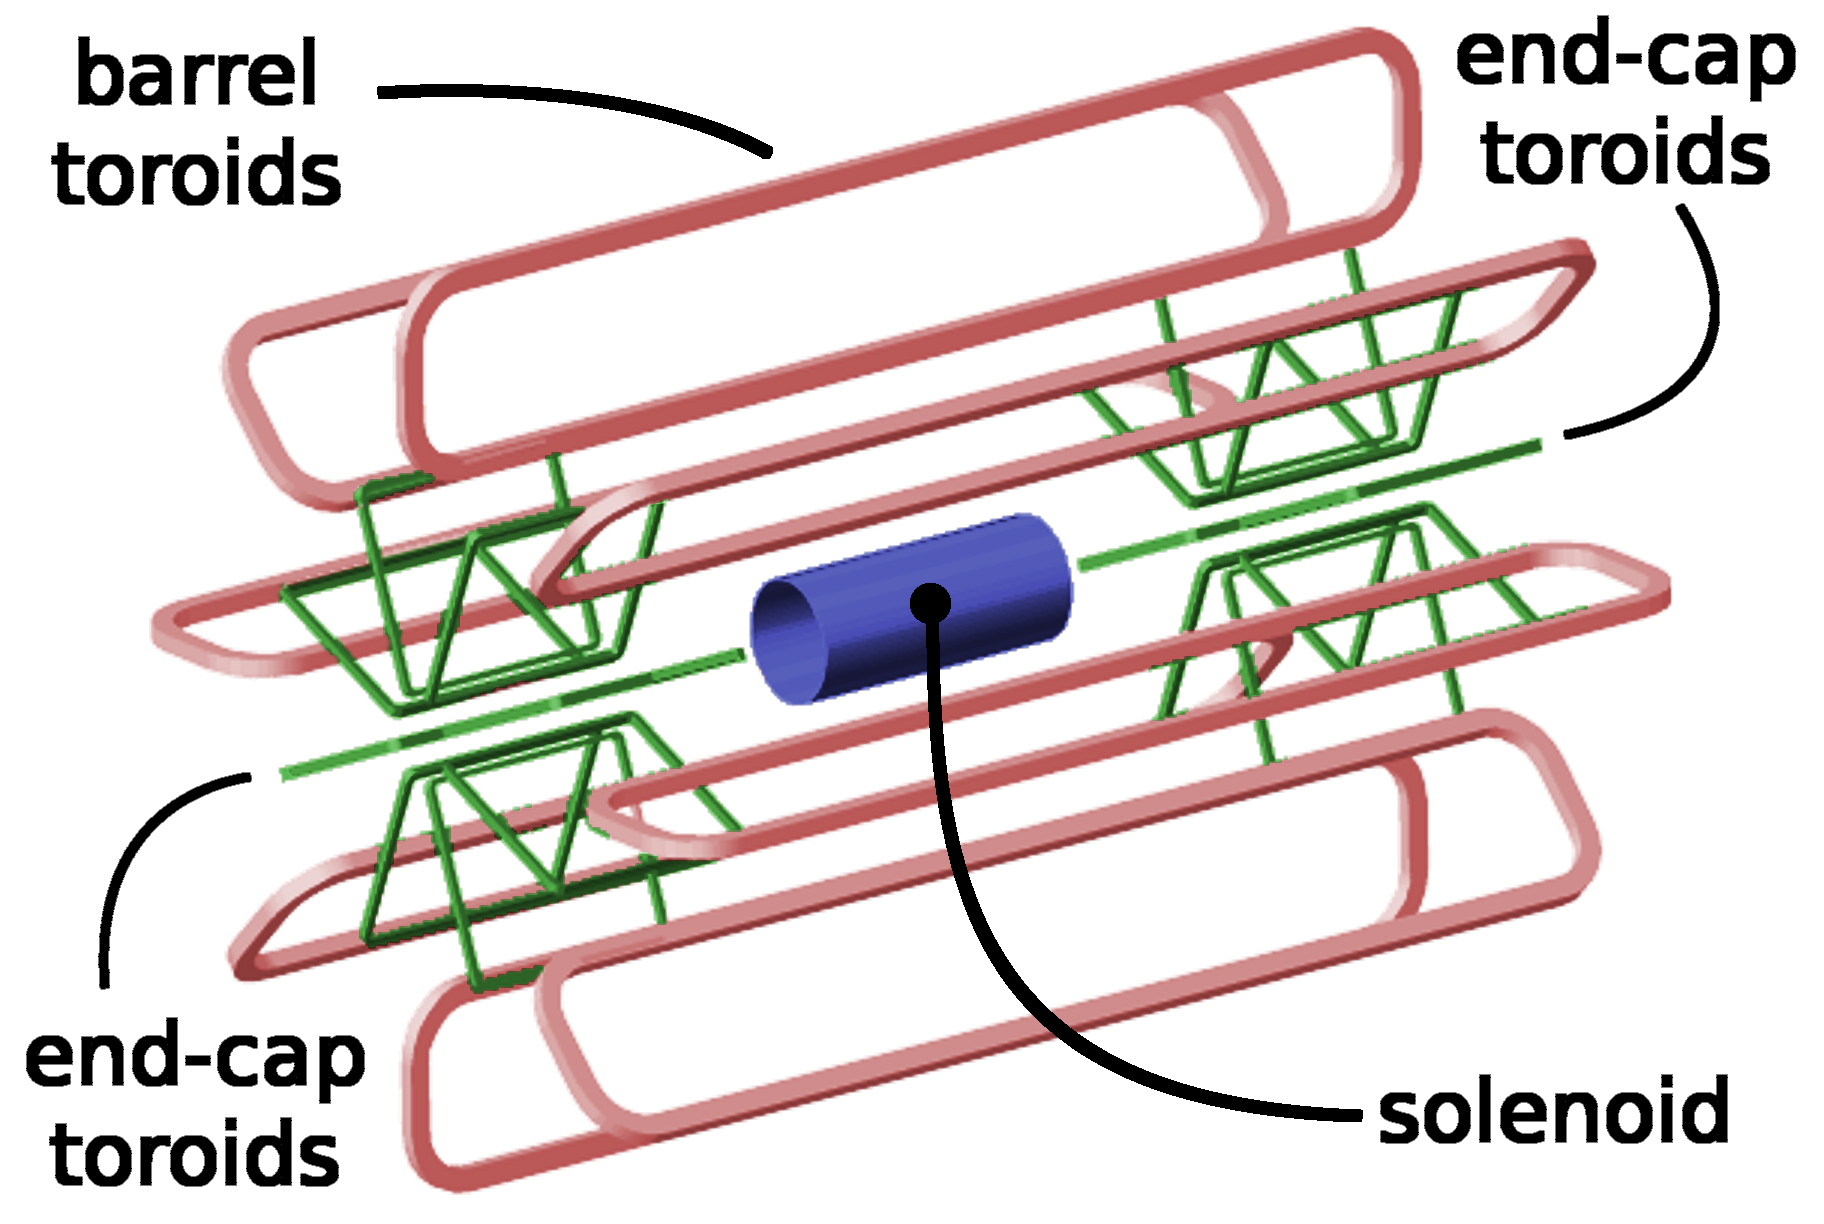
\includegraphics[width=.9\textwidth]{chapters/chapter2_experiment/images/magnetSystems.png}
    \caption{A schematic of the components of the magnet system in the ATLAS detector \cite{magnet-schematic}}
    \label{fig:magnetSystem}
\end{figure}

\begin{itemize}
    \item The central solenoid provides a 2 Tesla magnetic field. It is fitted between the \gls{ID} and the \gls{EM} calorimeter. Arising from a solenoid, this field is axially symmetric, and causes curvature in charged particles as they move through the \gls{ID}. In order to minimize material before the calorimeters, it was designed to be thin, a single-layer coil wound with 1173 turns with Al-stabilized Nb/Ti conductor. It covers a length of 5.3 m along the beam axis and has an outer diameter of 2.63 m\cite{central-solenoid}.

    \item The barrel toroid is made up of eight coils of a flat racetrack shape, which provide a symmetric radial field toward the beam axis, with a peak of 3.9 T \cite{barrel-toroid}. The two end-cap toroids are also composed of eight coils, with a length of 5 m, outer diameter of 10.7 m and an inner bore of 1.65 m, and providing a peak 4.1 T field. The end-cap toroids are inserted into the barrel toroid and line up with the center solenoid. The three-toroid design was chosen over a single toroid to maintain easy access to the core of the detector \cite{endcap-toroid}. Together the toroids provide a magnetic field to the muon system, causing curvature in the muon trajectory.
\end{itemize}


\subsection{Inner Detector}
The \gls{ID} serves to identify the precise interaction point and trajectory of charged particles. The \gls{ID} is segmented into barrel and endcap sections along the beam axis. The barrel extends 1.6 m, covering $|\eta| < 1$, and the endcap sectons cover the remainder of the 7 m length. With this setup, the \gls{ID} provides precision tracking up to $|\eta| = 2.5$ \cite{inner-detector-tdr}. It is composed of three subsystems, the Pixel Detector, the \gls{SCT}, and the \gls{TRT}. 

\begin{itemize}
    \item Pixel Detector: The pixel detector is comprised of four layers. The three outside pixel layers are comprised of a barrel-layer on the .  the innermost layer, the \gls{IBL}, takes advantage of smaller modules for finer granularity and . Each layer is comprised of modules with one sensor and sixteen readout chips.
    
    \item \gls{SCT}: The \gls{SCT} is composed of four layers . SCT modules are made of four strip sensors that are daisy-chained to one another.
\end{itemize}

\subsection{Calorimeters}
The calorimeter system in ATLAS serves to measure energy of particles absorbed by their active material. ATLAS employs calorimeters targeting different types of particle showering: the \gls{LAr} \gls{EM} calorimeter targets \gls{EM} showers from photons and electrons, while the hadronic Tile calorimeter targets hadronic showers. The \gls{EM} calorimeter lies outside the \gls{ID} and central solenoid, and the hadronic calorimeter is outside of the \gls{EM} calorimeter.  A schematic of the calorimeter can be found in Figure \ref{fig:calorimeter}.


\begin{figure}
    \centering
    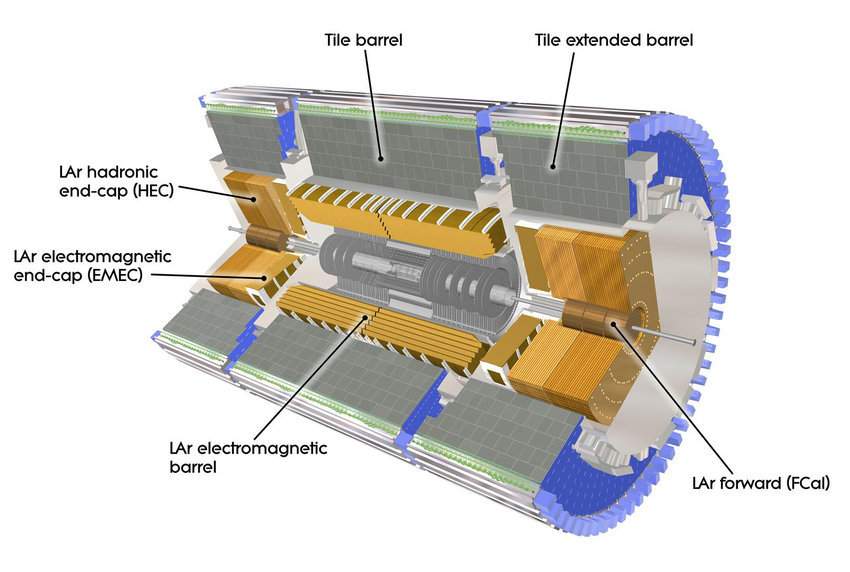
\includegraphics[width=.7\textwidth]{chapters/chapter2_experiment/images/calorimeter.jpeg}
    \caption{A schematic of the calorimeters in the ATLAS detector \cite{atlas-experiment}.}
    \label{fig:calorimeter}
\end{figure}

\begin{figure}
    \centering
    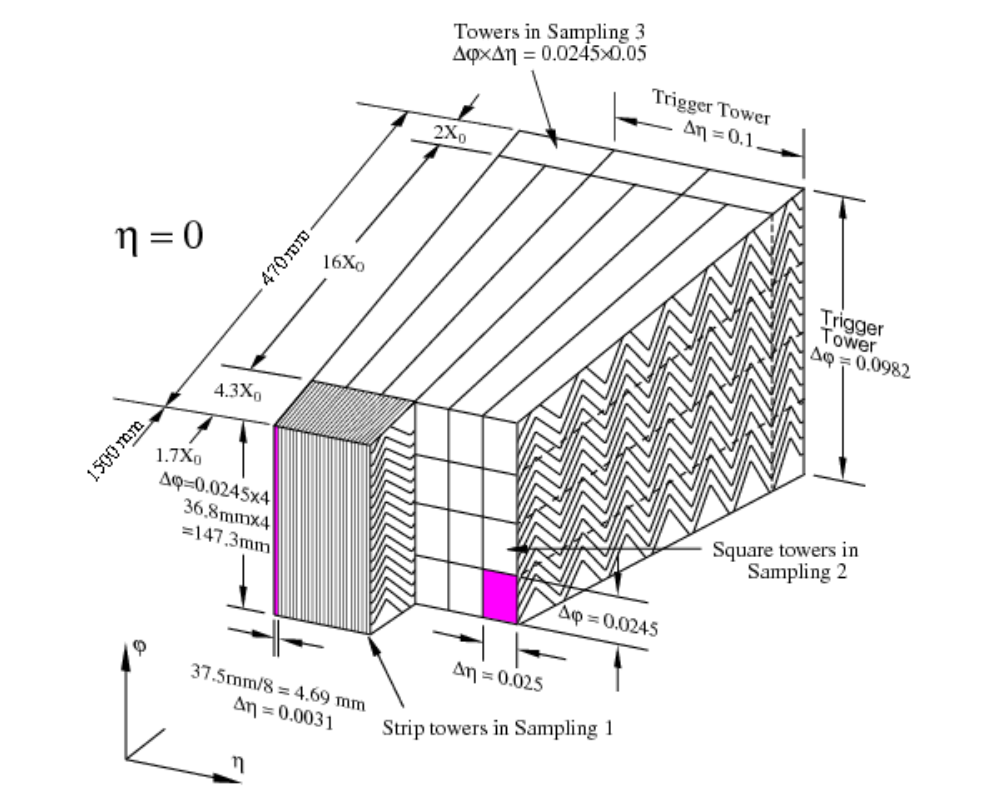
\includegraphics[width=.9\textwidth]{chapters/chapter2_experiment/images/lar.png}
    \caption{A sketch of the \gls{LAr} \gls{EM} calorimeter \cite{lar-tdr}.}
    \label{fig:lar}
\end{figure}

\noindent\textbf{Electromagnetic Calorimeter}\\
\indent The electromagnetic calorimeter is a \gls{LAr} sampling calorimeter. Upon interacting with the \gls{LAr} active material, photons will interact dominantly by creation of $e^+e^-$ pairs above 5 MeV. Below that threshold, photons interact via the photoelectric or Compton effect. For electrons, interaction occurs via bremsstrahlung at energies above 1 MeV, causing the electron to radiate photons and decelerate. This continues for subsequent daughter particles and has a showering effect in the calorimeter \cite{detectors-for-radiation}.

The \gls{LAr} \gls{EM} calorimeter features absorbers with an "accordion" style geometry, and read-out electrodes. The accordion geometry provides gap-less azimuthal ($\phi$) symmetry. The \gls{EM} calorimeter is composed of three regions, the \gls{EMB} and two \glspl{EMEC}, each with their own cryostat. 
    
The \gls{EMB} uses lead-stainless steel converters as the passive material and covers $|\eta| < 1.5$. It is split into two half-barrels, meeting at $|\eta| = 0$, each with 1024 converters and electrodes. Longitudinally, the \gls{EMB} is divided into three layers. The first strip layer is very finely segmented in $\eta$ to provide precision position information, with granularity $0.003 \times 0.1$ in $\Delta\eta \times \Delta \phi$. The second layer has a wider segmentation, $0.025 \times 0.025$, and absorbs the bulk of the \gls{EM} shower. The last layer has even lower granularity in $\eta$, $0.05 \times 0.025$, and serves to pick up the \gls{EM} shower tails. In total, these three layers cover $>22$ \gls{X_0} and have 101,760 total channels.

The \gls{EMEC} also uses lead-stainless steel as the passive material and is comprised of two concentric wheels, an inner wheel covering $1.4 < |\eta| < 2.5$, and an outer wheel covering $2.5 < |\eta| < 3.2$, and covers $>24$ \gls{X_0}. Between the \gls{EMB} and \gls{EMEC}, a transition crack spans $1.37 < |\eta| < 1.52$, which is also used to service the detector. 

In front of the calorimeter cryostats, a presampler is used to correct for energy lost before particles reach the calorimeters. The presampler uses thin copper electrodes and \gls{LAr} as the active material, with a layer of 1 cm thickness in the barrel and 5 mm in the end-caps, and granularity of $0.025 \times 0.1$ in $\Delta\eta \times \Delta \phi$ \cite{lar-tdr}.


A sketch of the composition of the \gls{EM} calorimeter can be found in Figure \ref{fig:lar}.

\begin{figure}
    \centering
    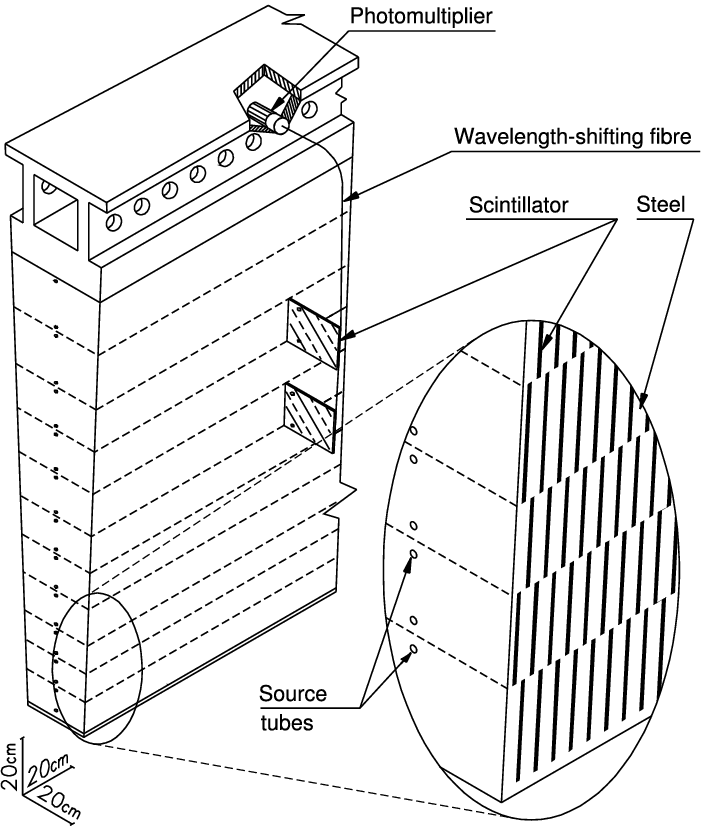
\includegraphics[width=.7\textwidth]{chapters/chapter2_experiment/images/tile.png}
    \caption{A sketch of the hadronic Tile calorimeter \cite{tile-tdr}.}
    \label{fig:tile}
\end{figure}


\noindent\textbf{Hadronic Calorimeter}\\ 
\indent When a hadron interacts with matter, both elastic scattering and inelastic interactions occur. Secondary hadrons are produced, including K and $\pi$ mesons, as well as protons and neutrons. These also decay and the cascade, known as a hadronic shower, will continue until the energy of the decay products is small enough to be halted by ionization energy loss or absorbed in a nuclear process \cite{detectors-for-radiation}.

\indent The hadronic Tile Calorimeter is designed to measure such decays, and using steel as the absorber and scintillating tiles as the active material. The scintillators transmit light via fiber optics to \glspl{PMT}. It is composed of three regions, the central barrel, covering $|\eta| < 1.0$, and two extended barrels on either side of the central barrel, covering $|\eta| > 1.0$. Each of these three regions have 64 azimuthal modules, and 3 layers longitudinally. The first two layers have granularity $0.1 \times 0.1$ in $\Delta\eta \times \Delta \phi$, while the third is $0.2 \times 0.1$. The thickness covers $>9.7$ \gls{intLen}. A sketch of the composition of the Tile Calorimeter can be seen in Figure \ref{fig:tile}.

A \gls{HEC} also works to detect hadronic decays, covering pseudorapidity range of $1.4 < |\eta| < 3.2$. There are two wheels per endcap, located behind the \glspl{EMEC} and sharing their cryostats. The \gls{HEC} uses \gls{LAr} as the active material, and copper plates as the passive material. Each end-cap features 32 wedge shaped modules, and two segments in depth, making four total samplings per endcap. \cite{lar-tdr}.

    
\noindent\textbf{\gls{FCal}}\\
\indent In order to get precise measurements of \gls{MET}, full $\eta$ coverage is necessary. The \gls{FCal} covers the most forward regions, covering $3.1 < |\eta| < 4.9$. It is three modules deep, covering 10 \gls{intLen}, the first module made of copper, targeting \gls{EM} depositions, and the outer two made of tungsten targeting hadronic depositions.



\subsection{Muon Spectrometer}

Timing information, useful for triggering, in the Muon Spectrometer is collected in the \glspl{RPC} and \glspl{TGC}. These both feature timing resolution better than 4.5 ns. The \glspl{RPC} cover the barrel ($|\eta| < 1.05$) region while the \glspl{TGC} covers the endcap ($1.0<|\eta|<2.4$).

\begin{figure}
    \centering
    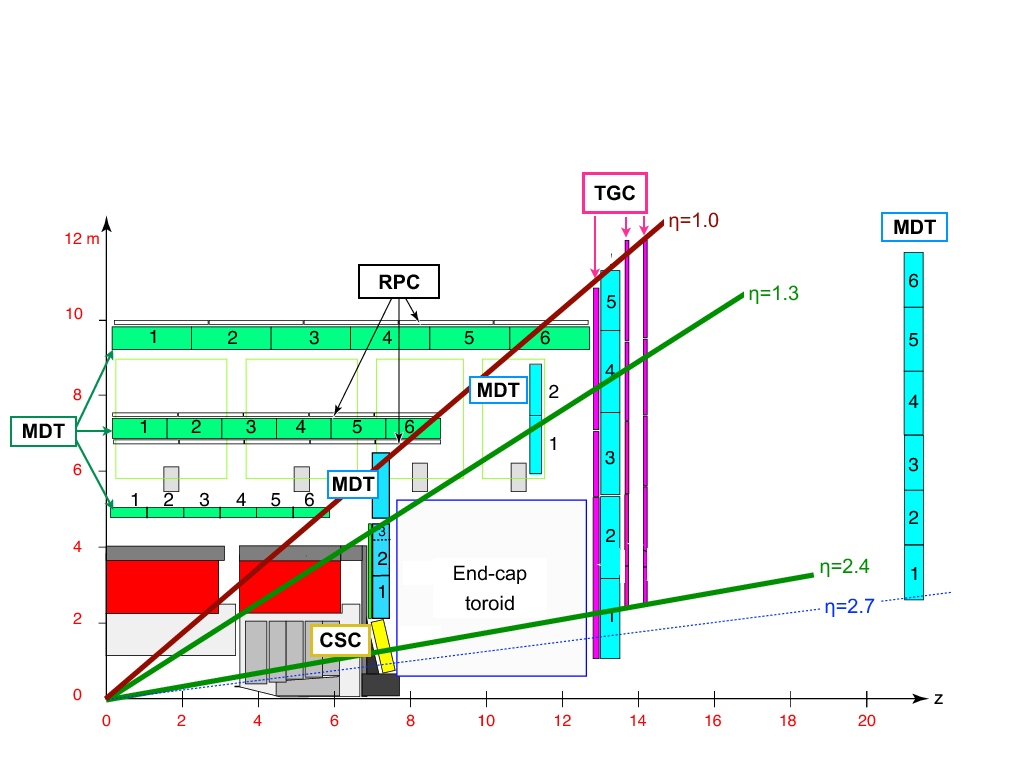
\includegraphics[width=.9\textwidth]{chapters/chapter2_experiment/images/muon_detector.png}
    \caption{A schematic of a quarter of the Muon Spectrometer. The described systems, the \gls{RPC}, \gls{TGC}, \gls{MDT}, and \gls{CSC} are labeled. \cite{muon-performance2015}.}
    \label{fig:muon-schematic}
\end{figure}


Momentum information is provided through Al tubes 30 mm in diameter and filled with a 0.05 mm gold-plated tungsten wire in the center, called a \gls{MDT}. Three layers of \glspl{MDT} cover the central region of the Muon Spectrometer, at $|\eta| < 2.7$. In the forward region, $2.0<|\eta|<2.7$, the first \glspl{MDT} layer is replaced by multi-wire proportional chambers with precision cathode strips, known as \glspl{CSC}.

A schematic of the Muon Spectrometer is found in Figure \ref{fig:muon-schematic}.

\subsection{Trigger and Data-Acquisition}

Dataflow and storage are a major challenge for ATLAS. Bunches of protons interact every 25 ns, a rate of 40 MHz. On average, raw event contains about 1.6 MB \cite{ATLASfact-sheet}, recording all of those interactions would not be possible, so to isolate events which contain interesting physics, ATLAS utilizes a two-stage trigger system.

First, the \gls{L1} trigger recieves events at 40 MHz and makes quick decisions based on coarse information. This trigger system is hardware based, constructed out of custom electronics, and targets specific features in the calorimeter or muon system. From hits in each detector, candidate physics objects (electrons, photons, muons, jets, and \gls{MET}) are formed, and then events are accepted or rejected based on features of these candidates in order to get to an average event rate of between 75 and 100 kHz, a reduction factor of about 400.

The second stage of the trigger is software-based, known the \gls{HLT}. The \gls{HLT} itself is composed of two steps, the \gls{L2} trigger system and the \gls{EF}. \gls{L1} accepted events are passed to a computing farm, then split into \glspl{ROI}, which are cones in $\eta \times \phi$. The design rate of the \gls{L2} trigger

Events that pass the \gls{L2} trigger are passed to the \gls{EF}, which reconstructs physics objects as close to offline reconstruction as possible, and then selects events using those objects. After the \gls{EF}, the final output is between 500 and 1000 Hz.
